\documentclass{beamer}
\usecolortheme{wolverine}

% math stuff
\usepackage{amsmath}
\usepackage{amsthm}
\usepackage{amssymb}
\usepackage{xcolor}

\usepackage{float}
\usepackage{subcaption}

% to insert images
\usepackage{graphicx}

% to correctly insert stressed characters
\usepackage[T1]{fontenc}
\usepackage[utf8]{inputenc}

\usepackage{multirow}

% Bibliography
% \usepackage[style=alphabetic]{biblatex}
% \usepackage[nottoc]{tocbibind}
% \usepackage{bibentry}
% \setcounter{biburllcpenalty}{9000}
% \usepackage{nameref}
% \addbibresource{slides.bib}

% to put links in table of contents
\usepackage{hyperref}
\hypersetup{colorlinks=false, %set true if you want colored links
	linktoc=all,     %set to all if you
}

\usepackage{mathtools}

% Add symbols
% \usepackage{textcomp}

% Add command for Real and Z sets
% \usepackage{dsfont}
% \newcommand{\Rset}{$\mathds{R}$}
% \newcommand{\Zset}{$\mathds{Z}$}

% Code highlighting
% \usepackage{minted}
% \usemintedstyle{perldoc}
% \setminted{
%     frame=single,
%     breaklines,
% }

% tikz figures
% \usepackage{tikzit}
% \input{style.tikzstyles}

% number rounding
\usepackage{siunitx}
\sisetup{round-mode=places,round-precision=5}

\definecolor{myyellow}{RGB}{225, 225, 0}

\title{Thesis notes}
\date{20th April}

% any code between @(...)@ is escaped back to LaTeX
% \lstset{escapeinside={@(}{)@}}

% algorithms
\usepackage[ruled,vlined]{algorithm2e}
% \newtheorem{theorem}{Theorem}

\begin{document}

\frame{\titlepage}

\begin{frame}[c]
	\frametitle{The Echo Chamber Problem - notation}

	\begin{itemize}
		\item $G = (V, E ^{+}, E ^{-}) $ interaction graph
		\item $ \mathcal{C} $ set of contents
		\item $C \in \mathcal{C} $ content, $\mathcal{T} _{C} $ set of threads
		      associated with $C$. A thread $T \in \mathcal{T} _{C} $ is a
		      subgraph of $G$
		      % So $G = \bigcup _{C
		      % \in \mathcal{C} } \bigcup _{T \in \mathcal{T} _C} T $ union of all
		      % threads of all contents
		\item $U \subseteq V$ subset of users, $T[U]$ subgraph of $T$ induced
		      by $U$. $|T(U)|$ is the number of edges of this subgraph
	\end{itemize}
\end{frame}

\begin{frame}[c]
	\frametitle{The Echo Chamber Problem - notation}
	\begin{itemize}
		\item $\eta(C)$ fraction of negative edges associated with $C$
		      (analogous definition for a thread $T$). Content (or thread)
		      controversial if $\eta \in [\alpha, 1]$
		\item $\hat{\mathcal{C} } \subseteq \mathcal{C} $ set of \textit{controversial}
		      contents

		\item $\mathcal{S} _C (U)$ set of \textit{non controversial} threads
		      induced by $U$, for \textit{controversial} contents, i.e.

			      {\small
				      \begin{equation}
					      \mathcal{S} _{C} (U) = \{ T[U] \; s.t. \; T[U] \; non \;
					      controversial, T \in \mathcal{T} _{C}, C
					      \in \hat{\mathcal{C}}, U \subseteq V\}
				      \end{equation}
			      }
	\end{itemize}

\end{frame}

\begin{frame}[c]
	\frametitle{The Echo Chamber Problem}
	\textbf{Goal}: given an interaction graph $G$, find $U \subseteq V$ maximing

	\begin{equation}
		\xi (U) = \sum^{}_{C \in \hat{\mathcal{C}} } \sum^{}_{T[U] \in S_C (U)}
		| T[U] |
	\end{equation}

	The set of users maximing the expression is denoted as $\hat{U}$ and the
	corresponding score is $\xi(G)$
\end{frame}

\begin{frame}[c]
	\frametitle{The Densest Echo Chamber Problem}
	\textbf{Goal}: given an interaction graph $G$, find $U \subseteq V$ maximing

	\begin{equation}
		\psi (U) = \sum^{}_{C \in \hat{\mathcal{C}} } \sum^{}_{T[U] \in S_C (U)}
		\frac{| T[U] |}{|U|}
	\end{equation}

	The set of users maximing the expression is denoted as $\hat{U}$ and the
	corresponding score is $\psi(G)$
\end{frame}




\begin{frame}[c]
	\frametitle{Unapproximable variations on the Echo Chamber problem}
	For any of these functions it is possible to find a number of negative
	edges to insert $s.t.$ the problem resorts to the original one

	\begin{equation*}
		\xi(U) = \sum^{}_{C \in \mathcal{C} } \sum^{}_{T \in \mathcal{T}_{C}  }
		(\alpha - \eta(T[U])) |T[U]|
	\end{equation*}

	\begin{equation*}
		\xi(U) = \sum^{}_{C \in \mathcal{C} } \sum^{}_{T \in \mathcal{T}_{C}  }
		(1 - \eta(T[U])) |T[U]|
	\end{equation*}

	\begin{equation*}
		\xi(U) = \sum^{}_{C \in \mathcal{C} } \sum^{}_{T \in \mathcal{T}_{C}  }
		(1 - \eta(T[U]))^{2}  |T[U]|
	\end{equation*}

	Same conclusion for the corresponding Densest version

\end{frame}

\begin{frame}[c]
	\frametitle{A solvable Densest Echo Chamber problem (1)}
	Let $G = (V, E)$ be the interaction graph, $\delta(i, j)$ and $\delta^{-} (i, j)$ the sum of the
	edges and negative edges, respectively, between vertices $v_{i} $ and
	$v_{j} $ associated to controversial contents.

	\bigskip

	The graph $G_d = (V_{d}, E_{d}) $ is constructed as follows from G:

	\begin{itemize}
		\item for any vertex $v_{i} \in V$ add a corresponding vertex in $V_{d} $
		\item for any pair of vertices in $G $
		      \begin{itemize}
			      \item let $\eta(i,j) \coloneqq \frac{\delta^{-} (i,j)}{\delta
					            (i,j)} $. If $\eta(i,j) \leq \alpha $ add a positive
			            edge between $v_{i} $ and $v_{j} $ in $G_{d} $
			            % \item don't add any edge otherwise between $v_{i} $ and $v_{j} $
		      \end{itemize}
	\end{itemize}

	Let $E_{d} [U]$ the set of edges induced on $G_d$ by $U \subseteq V$. \textbf{Goal}: find $U$ maximizing

	\begin{equation}
		\xi(U) = \frac{|E_{d} [U]|}{|U|}
	\end{equation}

\end{frame}

\begin{frame}[c]
	\frametitle{A solvable Densest Echo Chamber problem (2)}
	Alternatives:

	\begin{itemize}
		\item Compute DCS-AM on $G$, where each snapshot corresponds to a
		      content. Problems: graph may be too spars along contents, not
		      solvable in polynomial time.
		\item Aggregate edges separately for each $T \in T_{C}, C \in \hat{\mathcal{C}}$,
		      i.e. let $\delta_{T}(i,j) $ be $\delta(i, j)$ for the subgraph
		      $T$:
		      \begin{itemize}
			      \item let $\eta(T, i,j) \coloneqq \frac{\delta_{T} ^{-} (i,j)}{\delta
					            _{T} (i,j)} $. If $\eta(T, i,j) \leq \alpha $ add a positive
			            edge
		      \end{itemize}
	\end{itemize}
\end{frame}

\begin{frame}[c]
	\frametitle{A model for the Echo Chamber Problem}
	Model parameters:
	\begin{itemize}
		\item $b_{i} $, the group of each user $i$
		\item $\omega ^{+} _{rs} $ and $\omega ^{-} _{rs} $, the probabilities
		      of positive and negative edges, respectively, between users in
		      group $r$ and $s$ ($\omega ^{+} _{rs} + \omega ^{-} _{rs} \leq 1$).
	\end{itemize}

	For each node pairing $i, j$ consider their corresponding groups $r$ and
	$s$ and draw from the categorical distribution with parameters $(\omega _{rs} ^{+}, \omega
		_{rs} ^{-}, 1 - \omega _{rs} ^{+} - \omega _{rs} ^{-}) $ to add an edge (or
	not).
\end{frame}


\begin{frame}[c]
	\frametitle{Computing the score on the synthetic data (1)}

	The following graphs contains 2 communities of 40 vertices each and 10
	threads, for $\alpha = 0.2$. The results have been computed with the
	non-exact algorithm.
\end{frame}

\begin{frame}[c]
	\frametitle{Computing the score on the synthetic data (2)}
	First graph: mainly positive edges inside the groups and negative edges
	between groups.

	\begin{figure}
		\begin{center}
			\begin{subfigure}[b]{0.3\textwidth}
				\centering
				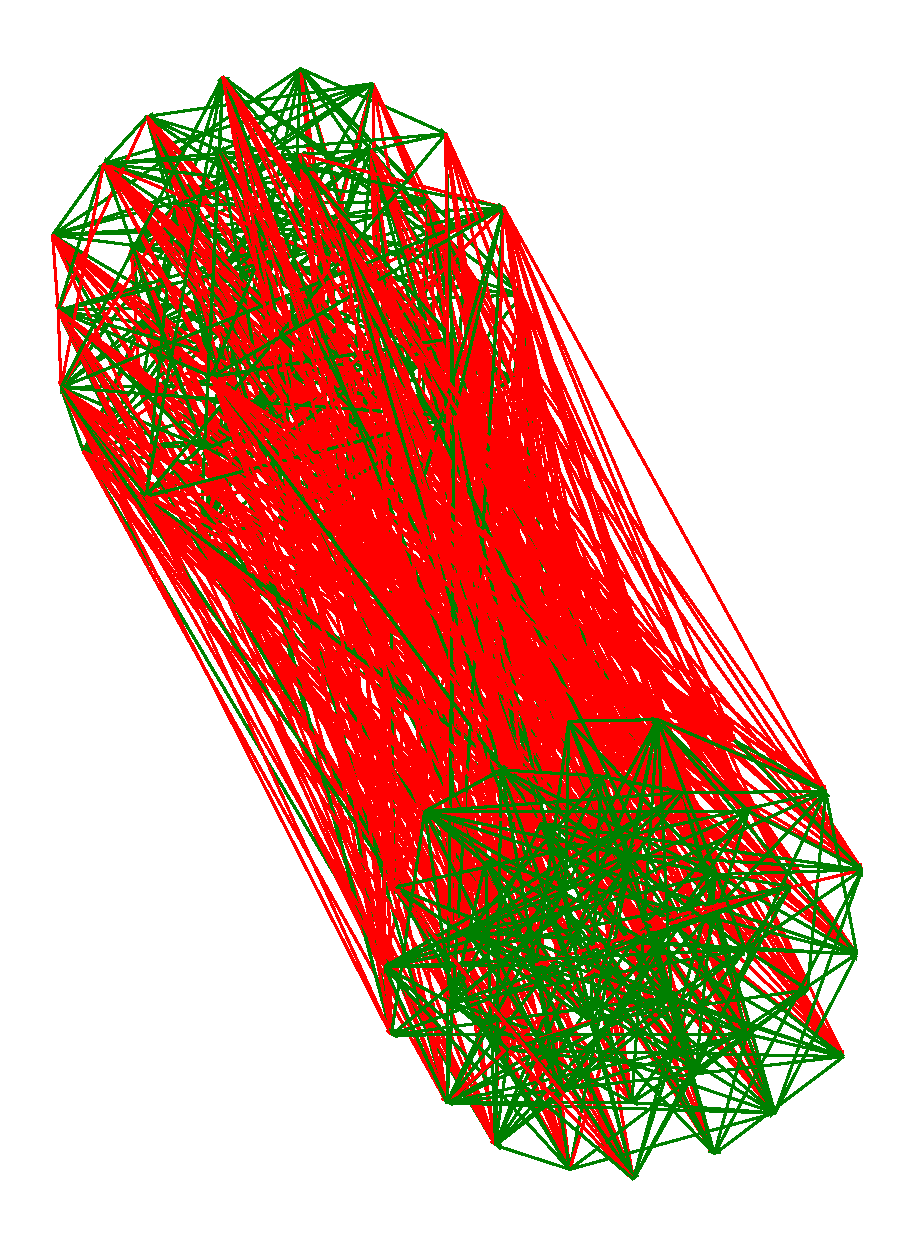
\includegraphics[width=\textwidth]{out/synthetic/graph1.pdf}
				\caption{Graph}
				\label{fig:}
			\end{subfigure}
			\begin{subfigure}[b]{0.3\textwidth}
				\centering
				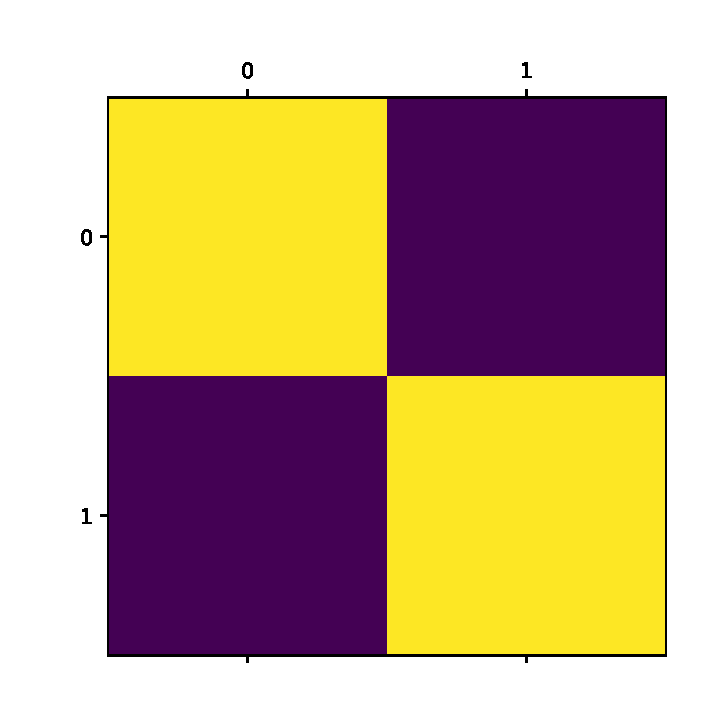
\includegraphics[width=\textwidth]{out/synthetic/omega_positive1.pdf}
				\caption{$\omega ^{+} _{rs} $}
				\label{fig:out/synthetic/omega_positive1.pdf}
			\end{subfigure}
			\begin{subfigure}[b]{0.3\textwidth}
				\centering
				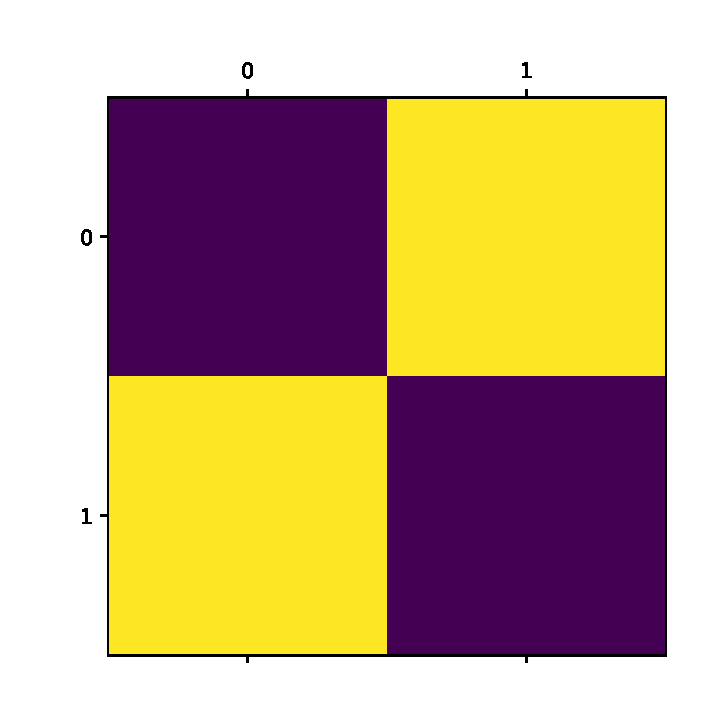
\includegraphics[width=\textwidth]{out/synthetic/omega_negative1.pdf}
				\caption{$\omega ^{-} _{rs} $}
				\label{fig:}
			\end{subfigure}
		\end{center}
	\end{figure}

	$|E| \approx 900, \; \eta(G) \approx 0.5, \; \bar{\xi}(G) = 32$.

	Time (single iteration): $8.5 $ seconds.
\end{frame}

\begin{frame}[c]
	\frametitle{Computing the score on the synthetic data (2)}
	Second graph: much more positive edges inside groups and negative edges
	between groups.

	\begin{figure}
		\begin{center}
			\begin{subfigure}[b]{0.3\textwidth}
				\centering
				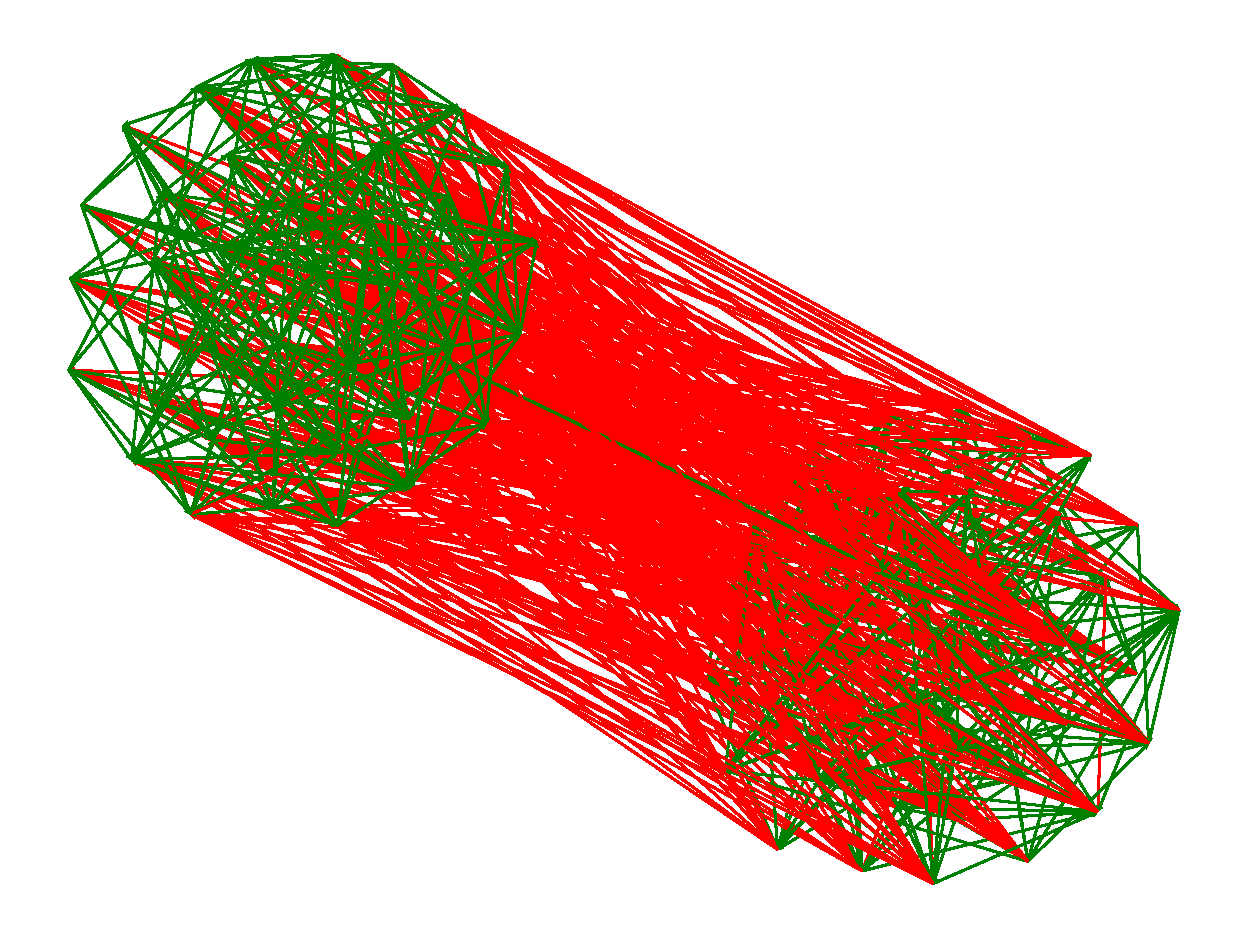
\includegraphics[width=\textwidth]{out/synthetic/graph2.pdf}
				\caption{Graph}
				\label{fig:}
			\end{subfigure}
			\begin{subfigure}[b]{0.3\textwidth}
				\centering
				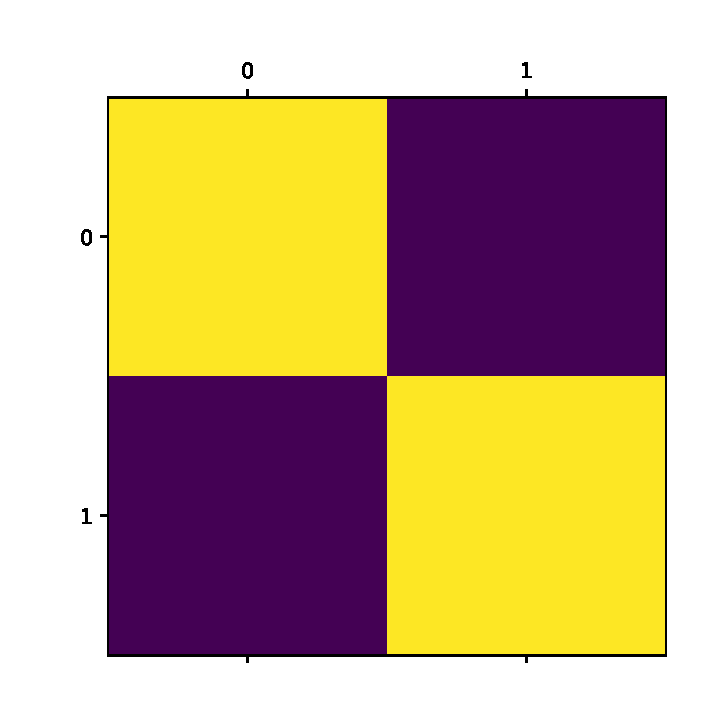
\includegraphics[width=\textwidth]{out/synthetic/omega_positive2.pdf}
				\caption{$\omega ^{+} _{rs} $}
				\label{fig:out/synthetic/omega_positive2.pdf}
			\end{subfigure}
			\begin{subfigure}[b]{0.3\textwidth}
				\centering
				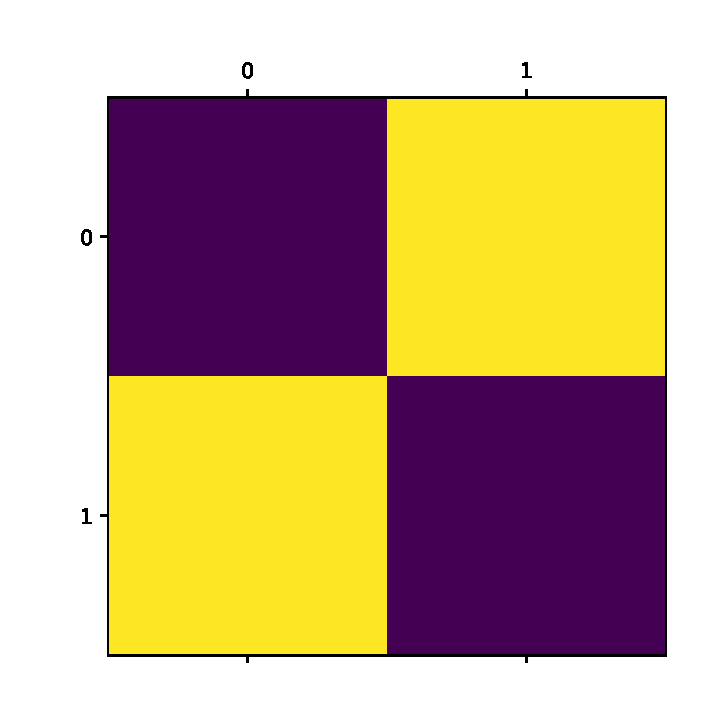
\includegraphics[width=\textwidth]{out/synthetic/omega_negative2.pdf}
				\caption{$\omega ^{-} _{rs} $}
				\label{fig:}
			\end{subfigure}
		\end{center}
	\end{figure}

	$|E| \approx 900, \; \eta(G) \approx 0.5, \; \bar{\xi}(G) = 96.6$.

	Time (single iteration): $8.9$ seconds.
\end{frame}

\begin{frame}[c]
	\frametitle{Computing the score on the synthetic data (2)}
	Third graph: equal distribution of positive and negative edges.

	\begin{figure}
		\begin{center}
			\begin{subfigure}[b]{0.3\textwidth}
				\centering
				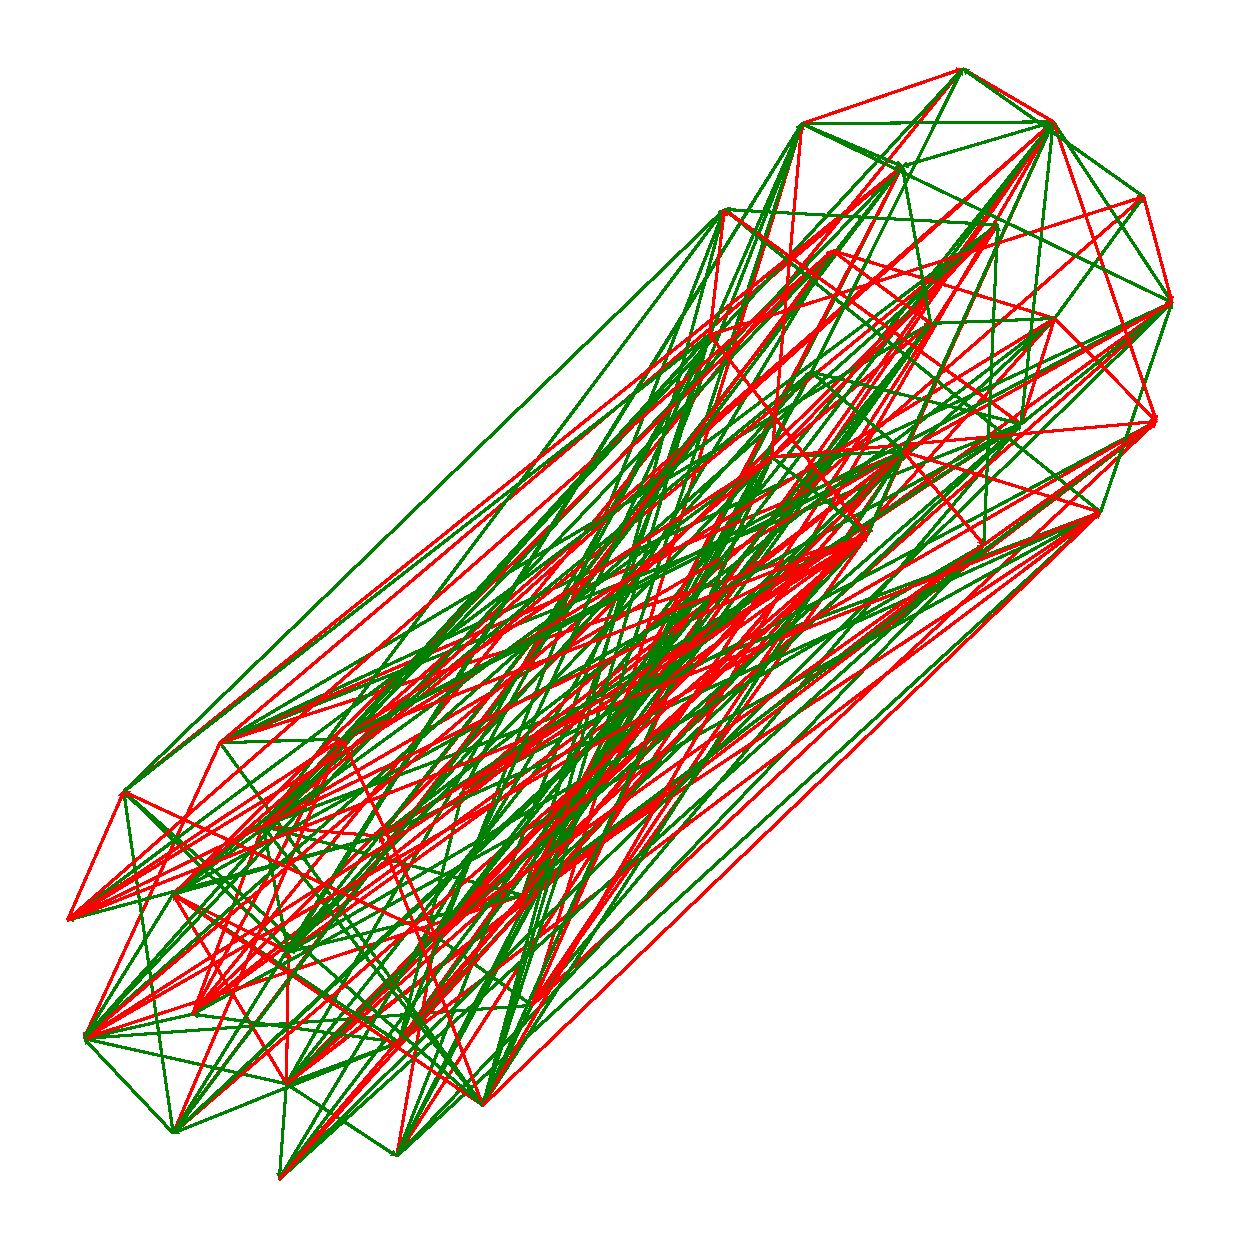
\includegraphics[width=\textwidth]{out/synthetic/graph3.pdf}
				\caption{Graph}
				\label{fig:}
			\end{subfigure}
			\begin{subfigure}[b]{0.3\textwidth}
				\centering
				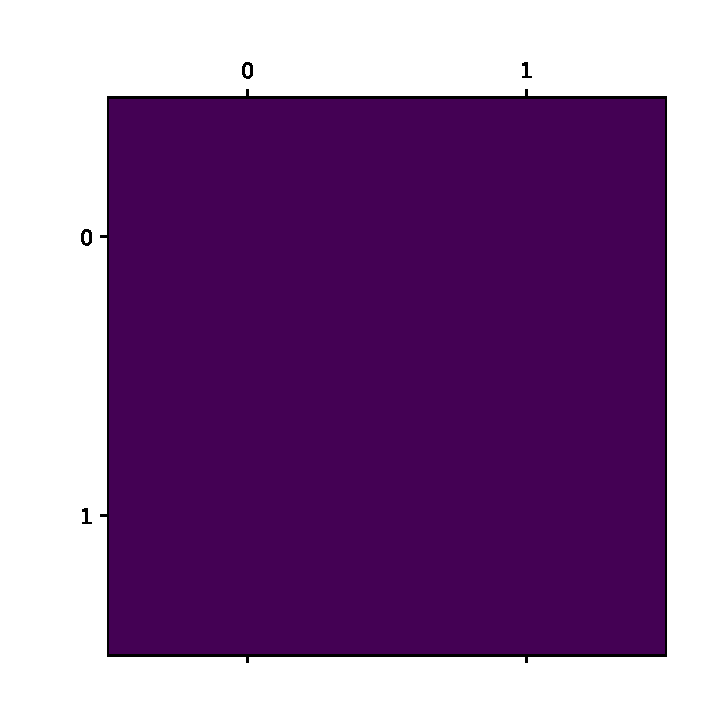
\includegraphics[width=\textwidth]{out/synthetic/omega_positive3.pdf}
				\caption{$\omega ^{+} _{rs} $}
				\label{fig:out/synthetic/omega_positive3.pdf}
			\end{subfigure}
			\begin{subfigure}[b]{0.3\textwidth}
				\centering
				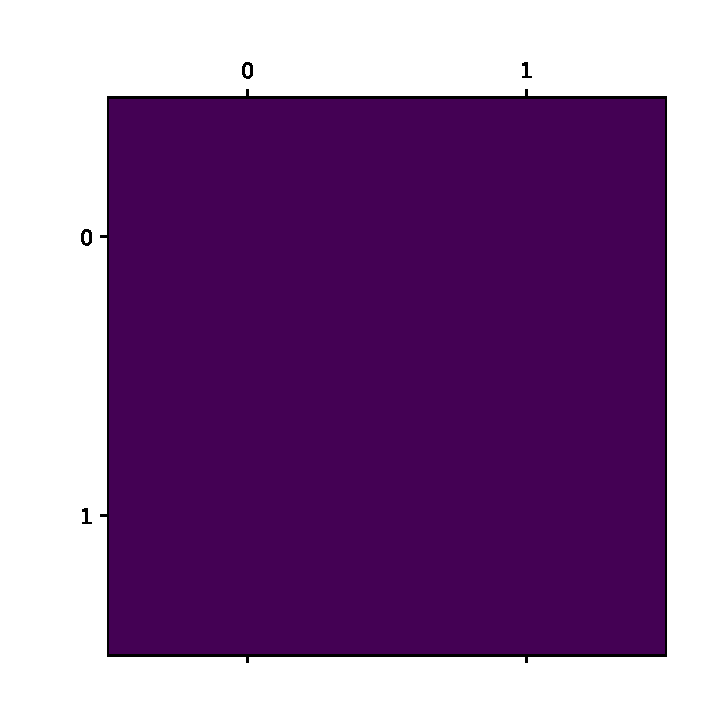
\includegraphics[width=\textwidth]{out/synthetic/omega_negative3.pdf}
				\caption{$\omega ^{-} _{rs} $}
				\label{fig:}
			\end{subfigure}
		\end{center}
	\end{figure}

	$|E| \approx 830, \; \eta(G) \approx 0.5, \; \bar{\xi}(G) = 19.8$.

	Time (single iteration): $8$ seconds.
\end{frame}

\begin{frame}[c]
	\frametitle{Computing the score on the synthetic data (4)}
	Fourth graph: positive and negative edges equally distributed in the
	graph but many more negative edges than positive ones.

	\begin{figure}
		\begin{center}
			\begin{subfigure}[b]{0.2\textwidth}
				\centering
				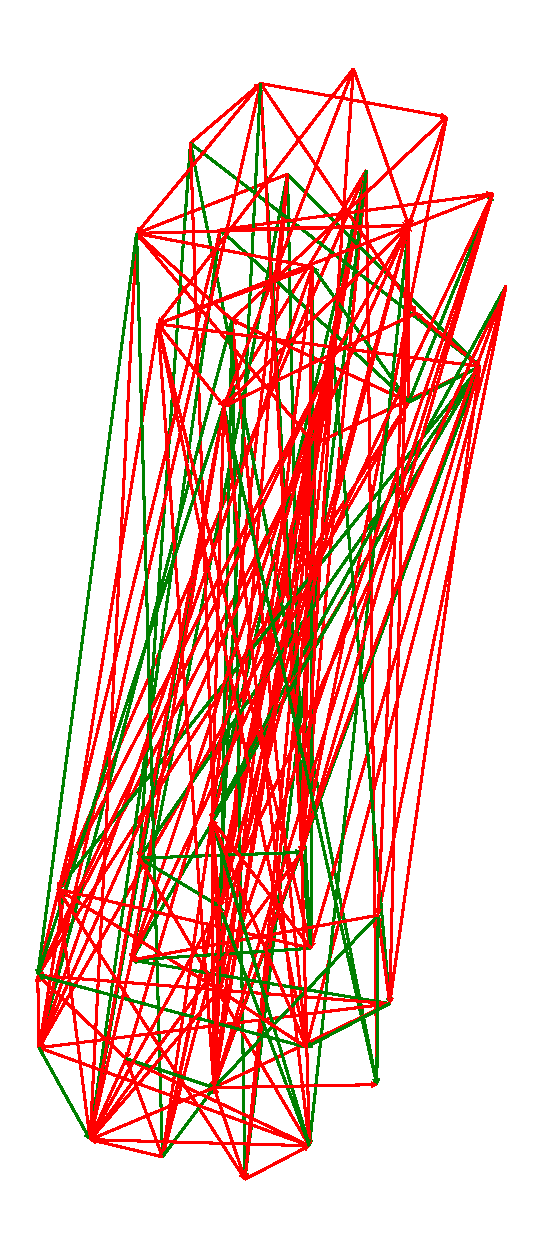
\includegraphics[width=\textwidth]{out/synthetic/graph4.pdf}
				\caption{Graph}
				\label{fig:}
			\end{subfigure}
			\begin{subfigure}[b]{0.2\textwidth}
				\centering
				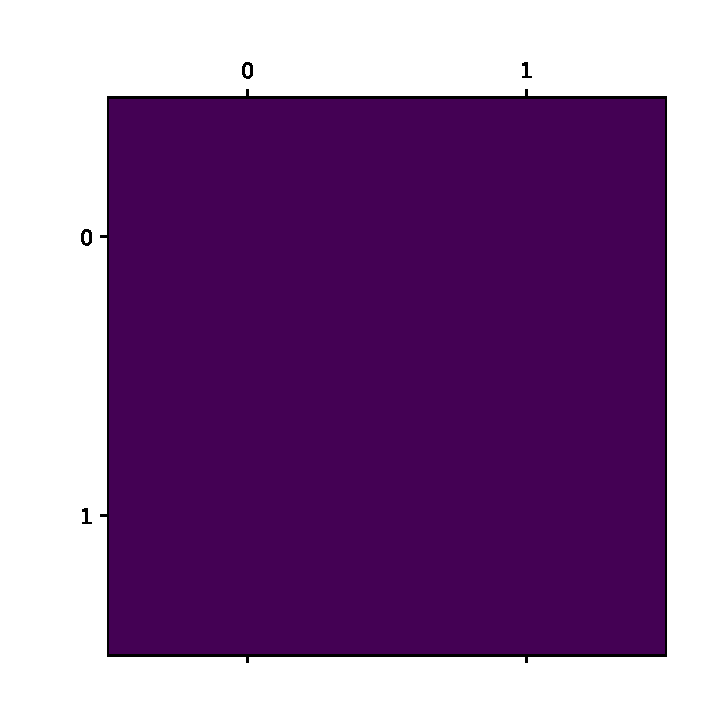
\includegraphics[width=\textwidth]{out/synthetic/omega_positive4.pdf}
				\caption{$\omega ^{+} _{rs} $}
				\label{fig:out/synthetic/omega_positive4.pdf}
			\end{subfigure}
			\begin{subfigure}[b]{0.2\textwidth}
				\centering
				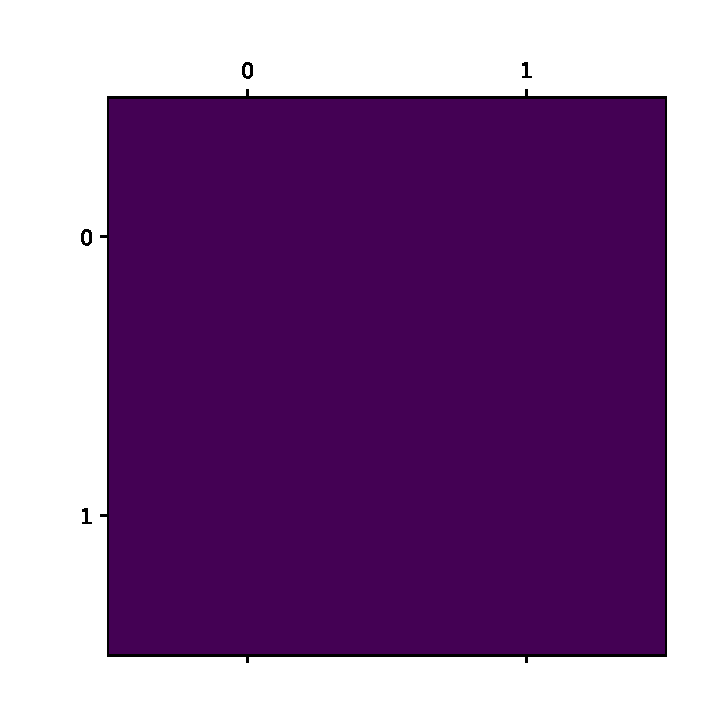
\includegraphics[width=\textwidth]{out/synthetic/omega_negative4.pdf}
				\caption{$\omega ^{-} _{rs} $}
				\label{fig:}
			\end{subfigure}
		\end{center}
	\end{figure}

	$|E| \approx 800, \; \eta(G) \approx 0.75, \; \bar{\xi}(G) = 9$.

	Time (single iteration): $7$ seconds.
\end{frame}

\begin{frame}[c]
	\frametitle{The datasets - negative edge fractions for contents}
	\begin{figure}
		\begin{center}
			\begin{subfigure}[b]{0.4\textwidth}
				\centering
				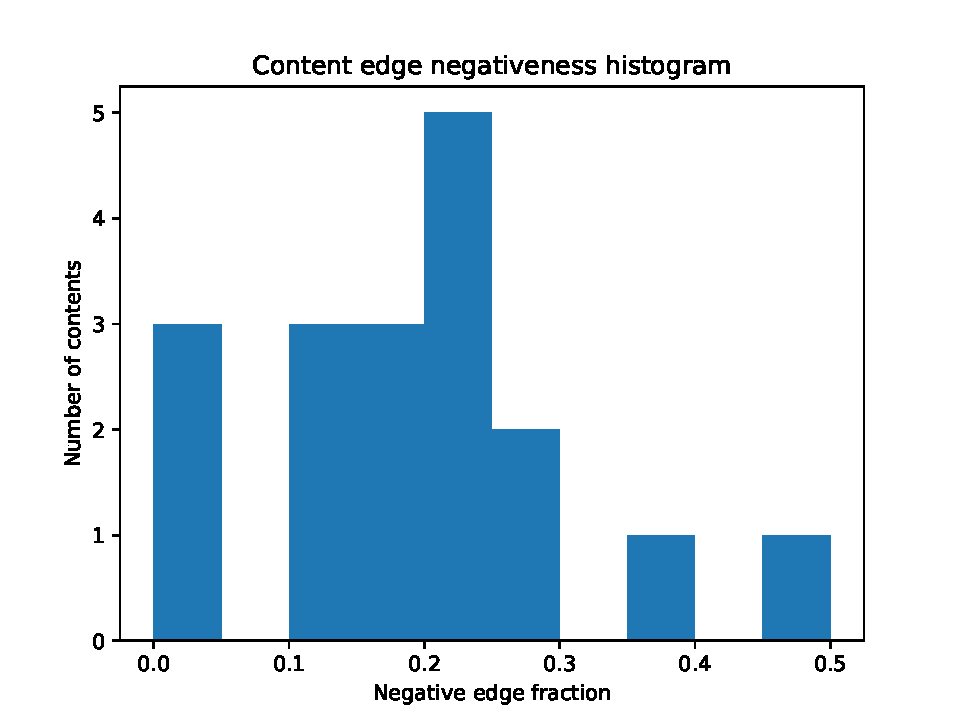
\includegraphics[width=\textwidth]{out/emanews200/neg-fraction-content-hist.pdf}
				\caption{@emanews}
				\label{fig:out/emanews200/neg-fraction-content-hist.pdf}
			\end{subfigure}
			\begin{subfigure}[b]{0.4\textwidth}
				\centering
				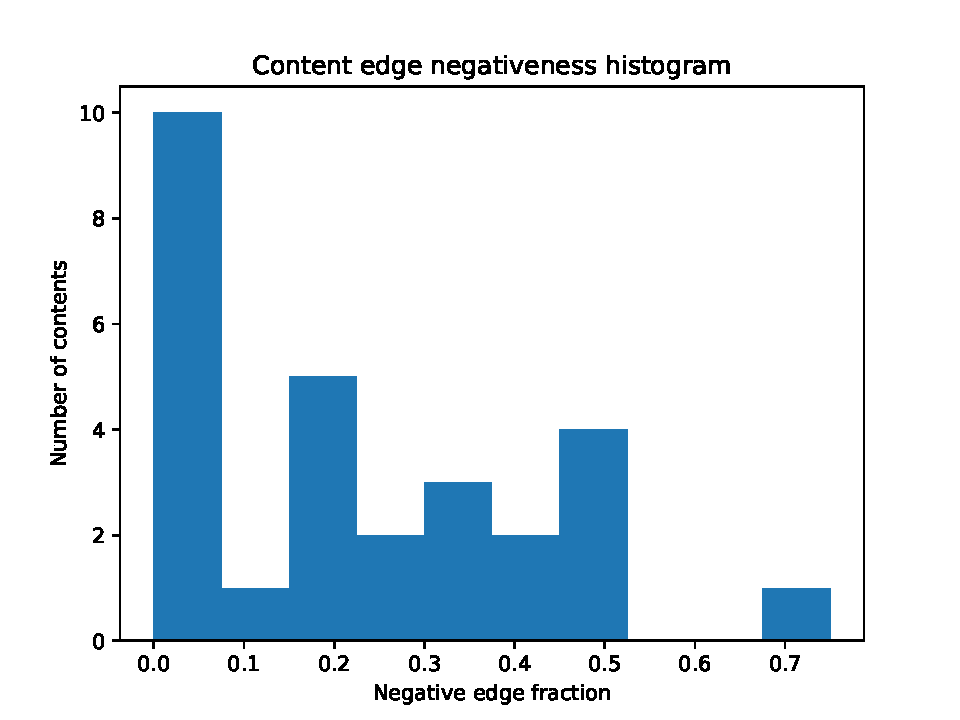
\includegraphics[width=\textwidth]{out/bbcscience200/neg-fraction-content-hist.pdf}
				\caption{@bbcscience}
				\label{fig:out/bbcscience200/neg-fraction-content-hist.pdf}
			\end{subfigure}
			\begin{subfigure}[b]{0.3\textwidth}
				\centering
				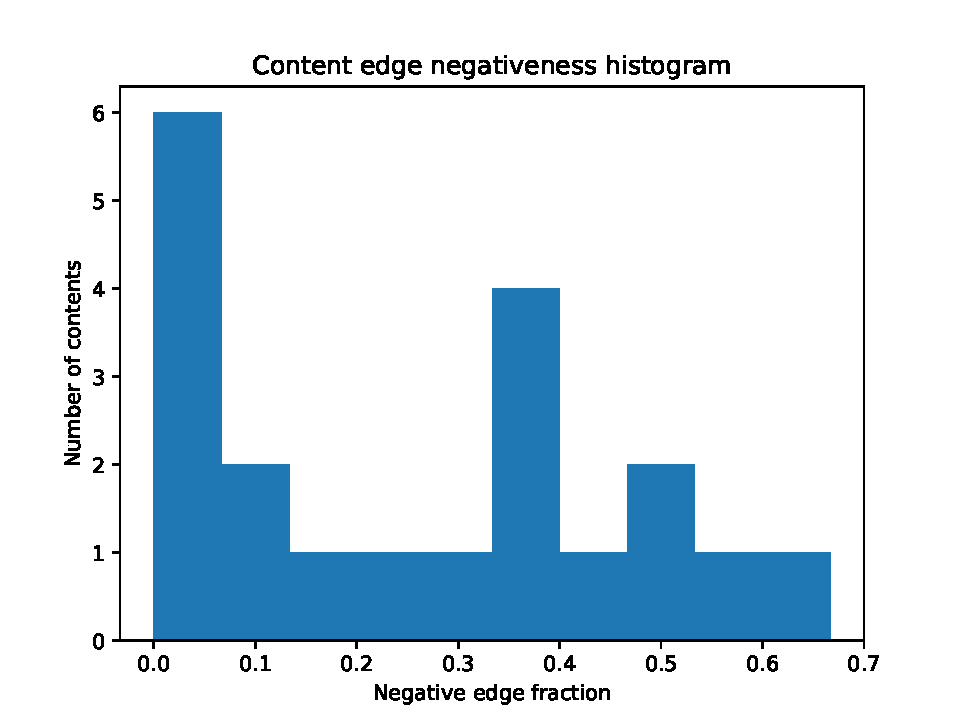
\includegraphics[width=\textwidth]{out/bbcentertainment200/neg-fraction-content-hist.pdf}
				\caption{@bbcentertainment}
				\label{fig:out/bbcscience200/neg-fraction-content-hist.pdf}
			\end{subfigure}
			\begin{subfigure}[b]{0.3\textwidth}
				\centering
				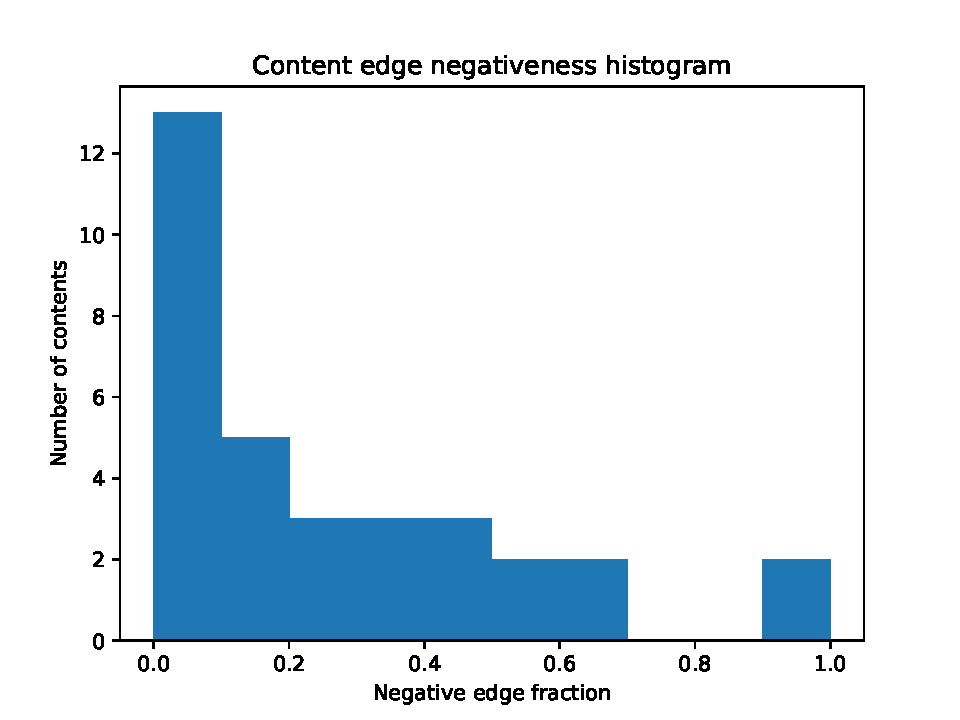
\includegraphics[width=\textwidth]{out/bbctech200/neg-fraction-content-hist.pdf}
				\caption{@bbctech}
				\label{fig:out/bbctech200/neg-fraction-content-hist.pdf}
			\end{subfigure}
			\begin{subfigure}[b]{0.3\textwidth}
				\centering
				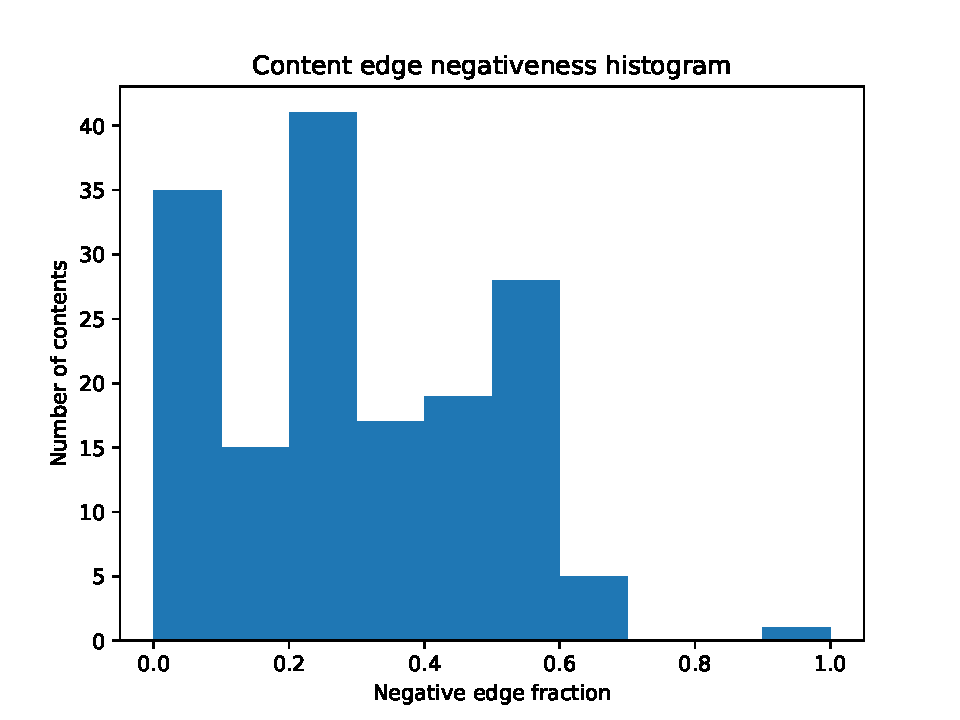
\includegraphics[width=\textwidth]{out/bbcsport200/neg-fraction-content-hist.pdf}
				\caption{@bbcsport}
				\label{fig:out/bbcsport200/neg-fraction-content-hist.pdf}
			\end{subfigure}
		\end{center}
	\end{figure}

\end{frame}


\begin{frame}[c]
	\frametitle{An initial implementation - results}

	\tiny{
		\begin{table}[htpb]
			\centering
			\caption{Echo chamber scores, MIP approaches. Each results is a tuple
				with (score, $|U|$, number of contributing threads, time in
				seconds)}
			\begin{tabular}{c|c|c|c}
				\textbf{Source, $|V|$, $|E|$} & $\xi_{MIP}(G) $      &
				$\xi_{MIPr\_alg}(G)$          & $\psi_{MIP} (G)$                                                \\
				\hline
				{@emanews, 1226, 1842}        & (0, 0, 0, 0.16)      & (0, 0, 0, 0.14)     & (0, 0, 0, 0.16)    \\
				{@bbcscience, 447, 388}       & (7, 12, 5, 0.09)     & (7, 12, 5, 0.05)    & (0.75, 4, 1, 0.11) \\
				{@bbcentertainment, 220, 183} & (34, 35, 6, 0.93)    & (34, 35, 6, 1.14)   & (1.5, 2, 1, 0.15)  \\
				{@bbctech, 713, 719}          & (309, 295, 30, 1.5)  & (309, 295, 30, 1.8) & (2.25, 4, 2, 0.76) \\
				{@bbcsport, 2140, 3100}       & (1030, 733, 48, 217) & (999,
				723, 46, 18.6)                & -                                                               \\
			\end{tabular}
		\end{table}
	}
\end{frame}
\end{document}
